\documentclass{article}

% Paquetes para mejor apariencia y personalización
\usepackage[spanish]{babel}
\usepackage[backend=bibtex,style=authoryear]{biblatex}
\usepackage{amsmath}
\numberwithin{equation}{section}
\usepackage[utf8]{inputenc}  % Codificación de caracteres
\usepackage{graphicx}        % Incluir imágenes
\usepackage{imakeidx}
\usepackage{hyperref}
%\usepackage{amsmath, amssymb, amsfonts}
%\usepackage{hyperref}
\makeindex[options=-c, intoc]
\hyphenation{vec-to-ria-les}
\hyphenation{e-xhaus-ti-va-men-te}
\hyphenation{a-cep-ta-ble}

\addbibresource{bibliografia.bib}

\begin{document}

% Generar la portada
\begin{titlepage}
    \centering
    {\Huge MÉTODOS PRELIMINARES DE DETERMINACIÓN DE ÓRBITAS A PARTIR DE OBSERVACIONES \\[1cm]}
    \vspace{1cm} % Espaciado opcional
    {\Large Víctor Ávila Camargo \\ 
    José Ignacio Miguel Rodríguez \\ 
    Javier Zaragozano Calvo \\[1cm]}
    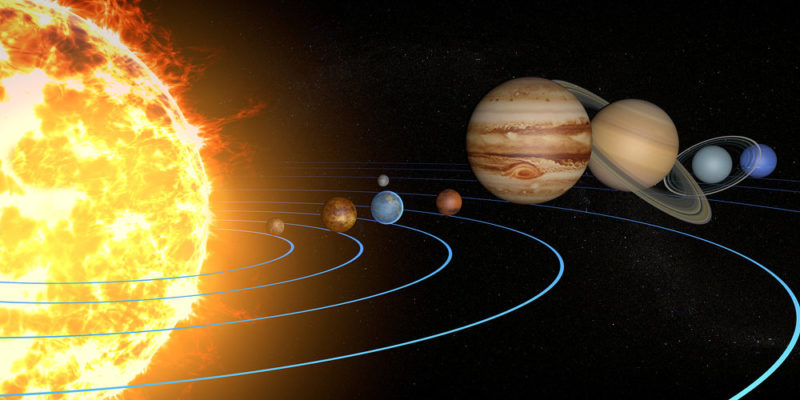
\includegraphics[width=1\textwidth]{orbitas-del-sistema-solar-e1555647256894.jpg} \\[1cm]
    
\includegraphics[width=0.1\textwidth]{aa.png} \\ [1cm]
    {\large \today}
\end{titlepage}
%\includegraphics[width=1\textwidth]{portada.jpg}
\newpage

\tableofcontents

\newpage

\begin{center}
\textbf{Abstract}\\
    En este artículo se abordarán varios métodos para determinar 
    los parámetros orbitales de la órbita de varios cuerpos celestes a partir de distintas observaciones.
\end{center}
\section{Introducción} %Motivación del problema
\index{Introducción}
Hoy en día y desde hace ya un tiempo, 
varios exoplanetas son descubiertos a diario, cada uno con sus propias características. 
Para terminar de caracterizarlos por completo, es necesario 
hacer un estudio de cómo es su órbita. Esto es importante porque estudiándola podemos recabar algunos 
datos que de otro modo sería imposible. 
Por ejemplo, podemos ver si el exoplaneta se encuentra en la zona habitable 
de su estrella o no, viendo qué tan grande es el periodo de su 
órbita. \\ 

Sin embargo, tomar una medida de su posición cada día sería 
algo tremendamente ineficiente. Es por eso que antiguos 
matemáticos y físicos desarrollaron algunos métodos para 
determinar su órbita de manera preliminar a partir de, generalmente, 
tres medidas. Algunos de estos métodos son el método de 
Gauss o el método de Gibbs. \\

Estos métodos han logrado varios hitos bastante importantes 
en la historia de la mecánica celeste. Uno de estos logros 
y quizás el más importante fue la determinación de la órbita 
del planeta enano Ceres. Este planeta enano fue descubierto 
el 1 de enero de 1801 por el astrónomo italiano Giuseppe Piazzi ($1746-1826$). 
Sin embargo, debido a su rápido movimiento, pronto le perdieron 
de vista y ahí es cuando aparece la gran aportación del matemático Carl Friedrich Gauss ($1777-1855$), 
que, con su método, calculó la órbita de Ceres a partir de 
las pocas observaciones que había de él en la época y, gracias 
a su alta precisión, pudieron volver a localizarle. \\

Una vez motivado el esfuerzo de dedicarle un artículo a los 
método de determinación de órbitas, vamos a comenzar desarrollando 
el aspecto más teórico de los dos métodos en los que nos 
vamos a centrar: El método de Gibbs y el método de Gauss.
\section{Método de Gibbs}
\index{Método de Gibbs}
Para este método es necesario conocer la posición de un cuerpo 
respecto al centro de atracción en 3 instantes de tiempo distintos, 
$t_{1}$, $t_{2}$ y $t_{3}$. A partir de estas tres posiciones, 
podremos obtener las velocidades $\overrightarrow{v_{1}}$, 
$\overrightarrow{v_{2}}$ y $\overrightarrow{v_{3}}$ suponiendo 
que nos encontramos en una órbita de dos cuerpos. La solución a 
este problema la obtuvo el americano J.W. Gibbs ($1839-1903$) 
usando simplemente un análisis vectorial. A continuación, 
entraremos más en detalle sobre cómo se deduce este método.
\subsection{Deducción del método de Gibbs}
Sabemos que por la conservación del momento angular, 
las posiciones de un cuerpo que orbita alrededor de otro se encuentran todas 
en el mismo plano. Entonces, partiendo de nuestras tres posiciones 
obtenidas en tres tiempos distintos, podemos calcular el 
vector unitario de $\overrightarrow{r_{1}}$ y otro vector 
unitario que sea resultado del producto vectorial de $r_{2}$ y 
$r_{3}$ del siguiente modo: 
\begin{align*}
    &\hat{u}_{r1}=\frac{\overrightarrow{r_{1}}}{r_{1}} \\
    &\hat{C}_{23}=\frac{\overrightarrow{r_{2}}\times \overrightarrow{r_{3}}}{\left\lVert \overrightarrow{r_{2}}\times \overrightarrow{r_{3}} \right\rVert }  
\end{align*}
Como $\overrightarrow{r_{1}}$, $\overrightarrow{r_{2}}$ y 
$\overrightarrow{r_{3}}$ están en el mismo plano, entonces: 
\begin{equation*}
    \hat{u}_{r1}\cdot \hat{C}_{23}=0
\end{equation*}
Además, como se ve en la siguiente figura, nosotros podemos 
expresar $\overrightarrow{r_{2}}$ como una combinación lineal 
de $\overrightarrow{r_{1}}$ y $\overrightarrow{r_{3}}$: 
\begin{equation}
    \overrightarrow{r_{2}}=\alpha \overrightarrow{r_{1}}+\beta \overrightarrow{r_{3}}
\end{equation}
\begin{figure}[h]
    \centering
    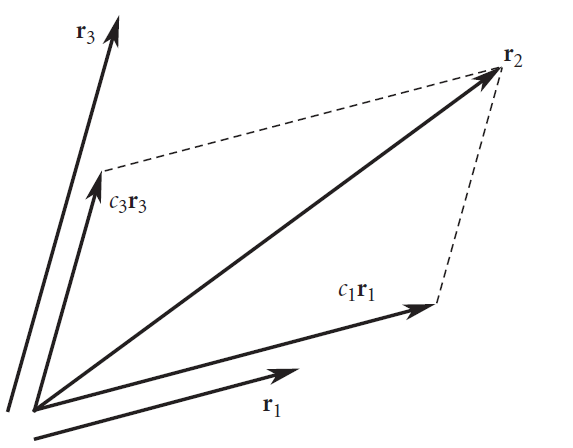
\includegraphics[width=0.6\textwidth]{a.png}
    \caption{Demostración de la ecuación 2.1 (Créditos 
    HowardD. Curtis)}
\end{figure} \\

Una vez tenemos estas consideraciones en mente ya podemos 
empezar a calcular las distintas velocidades. \\

Para calcularlas vamos a partir de la siguiente 
fórmula: 
\begin{equation}
    \overrightarrow{v}\times \overrightarrow{h}=\mu\left(\frac{\overrightarrow{r}}{r}+\overrightarrow{e}\right) 
\end{equation}
Donde $\overrightarrow{h}$ es el momento angular y 
$\overrightarrow{e}$ es el vector excentricidad. Para despejar 
$\overrightarrow{v}$ vamos a multiplicar vectorialmente a ambos 
lados por $\overrightarrow{h}$. Entonces, centrándonos de momento 
en lado izquierdo de la ecuación, obtenemos: 
\begin{equation*}
    \overrightarrow{h}\times(\overrightarrow{v}\times\overrightarrow{h})
\end{equation*}
Para continuar vamos a aplicar la siguiente propiedad del 
triple producto vectorial: $\overrightarrow{A}\times(\overrightarrow{B}\times\overrightarrow{C})
=(\overrightarrow{A}\cdot\overrightarrow{C})\overrightarrow{B}-(\overrightarrow{A}\cdot\overrightarrow{B})\overrightarrow{C}$
y obtenemos lo siguiente: 
\begin{equation*}
    \overrightarrow{h}\times(\overrightarrow{v}\times\overrightarrow{h})=(\overrightarrow{h}\cdot\overrightarrow{h})\overrightarrow{v}-(\overrightarrow{v}\cdot\overrightarrow{h})\overrightarrow{h}
\end{equation*}
Pero como $\overrightarrow{h}\cdot\overrightarrow{h}=h^{2}$ y 
$\overrightarrow{v}\perp\overrightarrow{h}$ obtenemos: 
\begin{equation*}
    \overrightarrow{h}\times(\overrightarrow{v}\times\overrightarrow{h})=h^{2}\overrightarrow{v}
\end{equation*}
Y nuestra ecuación 2.2 queda de la siguiente manera:
\begin{equation}
    \overrightarrow{v}=\frac{\mu}{h^{2}}\left(\frac{\overrightarrow{h}\times\overrightarrow{r}}{r}+\overrightarrow{h}\times\overrightarrow{e}\right)
\end{equation}
Cabe destacar que, en el sistema perifocal (sistema centrado en el foco de la elipse), el vector unidad 
$\hat{p}$ tiene la misma dirección que el vector 
de la excentricidad y el vector $\hat{w}$ es perpendicular 
al plano de la órbita en la dirección de $\overrightarrow{h}$. Por 
lo que, en el sistema perifocal, nuestra ecuación se transforma en: 
\begin{equation}
    \overrightarrow{v}=\frac{\mu}{h^{2}}\left(\frac{h\hat{w}\times\overrightarrow{r}}{r}+h\hat{w}\times e\hat{p}\right)=\frac{\mu}{h}\left[\frac{\hat{w}\times\overrightarrow{r}}{r}+e(\hat{w}\times\hat{p})\right]
\end{equation}
Como $\hat{w}$ y $\hat{p}$ son 2 vectores 
de la base en el sistema perifocal, entonces su producto 
vectorial será el tercer vector de la base ($\hat{q}$). 
Así que esto hace que nuestra ecuación se reduzca a: 
\begin{equation}
    \overrightarrow{v}=\frac{\mu}{h}\left(\frac{\hat{w}\times\overrightarrow{r}}{r}+e\hat{q}\right)
\end{equation}
Este es un resultado muy importante porque nos marca nuestro 
camino a seguir. Necesitamos encontrar una forma de obtener 
los vectores y magnitudes $\hat{p}$, $\hat{q}$, 
$\hat{w}$, $h$ y $e$ a partir de nuestros tres 
vectores de posiciones y así poder aplicar la fórmula 2.5. \\

Como nuestros tres vectores de posición son parte de una 
órbita, podemos multiplicar a nuestra ecuación 2.1 por el 
vector excentricidad y obtener: 
\begin{equation*}
    \overrightarrow{r_{2}}\cdot\overrightarrow{e}=\alpha\overrightarrow{r_{1}}\cdot\overrightarrow{e}+\beta\overrightarrow{r_{3}}\cdot\overrightarrow{e}
\end{equation*} 
Estos productos escalares dan como resultado: 
\begin{equation}
    \overrightarrow{r_{i}}\cdot\overrightarrow{e}=\frac{h^{2}}{\mu}-r_{i} 
\end{equation}
Por lo que si lo sustituimos todo al final llegamos a:
\begin{equation}
    \frac{h^{2}}{\mu}-r_{2}=\alpha\left(\frac{h^{2}}{\mu}-r_{1}\right)+\beta\left(\frac{h^{2}}{\mu}-r_{3}\right)
\end{equation}
Ahora, nuestro objetivo es eliminar los coeficientes $\alpha$ 
y $\beta$ por lo que, para ello, vamos a multiplicar vectorialmente 
a nuestra ecuación 2.1 por $\overrightarrow{r_{1}}$ y 
por $\overrightarrow{r_{3}}$ obteniendo así:
\begin{align*}
    &\overrightarrow{r_{2}}\times\overrightarrow{r_1}=\beta(\overrightarrow{r_{3}}\times\overrightarrow{r_{1}})   &\overrightarrow{r_{2}}\times\overrightarrow{r_3}=-\alpha(\overrightarrow{r_{3}}\times\overrightarrow{r_{1}})
\end{align*}
Con este resultado en mente, si multiplicamos a nuestra ecuación 
2.7 por el producto vectorial de $\overrightarrow{r_3}$ y 
$\overrightarrow{r_1}$ vamos a obtener:
\begin{equation*}
    \frac{h^{2}}{\mu}(\overrightarrow{r_{3}}\times\overrightarrow{r_{1}})-r_{2}(\overrightarrow{r_{3}}\times\overrightarrow{r_{1}})=-(\overrightarrow{r_{2}}\times\overrightarrow{r_{3}})\left(\frac{h^{2}}{\mu}-r_{1} \right)+(\overrightarrow{r_{2}}\times\overrightarrow{r_{1}})\left(\frac{h^{2}}{\mu}-r_{3} \right)
\end{equation*}
Gracias a esto, hemos podido eliminar los coeficientes 
$\alpha$ y $\beta$. Si agrupamos términos al final obtenemos: 
\begin{equation*}
    \frac{h^{2}}{\mu}(\overrightarrow{r_{1}}\times\overrightarrow{r_{2}}+\overrightarrow{r_{2}}\times\overrightarrow{r_{3}}+\overrightarrow{r_{3}}\times\overrightarrow{r_{1}})=r_{1}(\overrightarrow{r_{2}}\times\overrightarrow{r_{3}})+r_{2}(\overrightarrow{r_{3}}\times\overrightarrow{r_{1}})+r_{3}(\overrightarrow{r_{1}}\times\overrightarrow{r_{2}}) 
\end{equation*}
Para poner esta ecuación de un modo más simple, vamos a llamar 
al paréntesis de la izquierda $\overrightarrow{D}$ y a la 
parte de la derecha $\overrightarrow{N}$. Entonces: 
\begin{equation}
    \overrightarrow{N}=\frac{h^{2}}{\mu}\overrightarrow{D} 
\end{equation}
Poniendo esta ecuación en función de los módulos N y D (esencialmente 
es la misma ecuación), podemos despejar h y obtener: 
\begin{equation}
    h=\sqrt{\mu\frac{N}{D}}
\end{equation}
Como N y D dependen solo de los vectores de posición ya hemos 
conseguido uno de nuestros objetivos, el de obtener h a partir 
de los vectores de posición. Además, como todos los vectores son  coplanarios, todos sus productos vectoriales van a ser perpendiculares  al plano de la órbita, pudiendo definir: 
\begin{equation}
    \hat{w}=\frac{\overrightarrow{D}}{D} 
\end{equation}
Ya tenemos $\hat{w}$ en función de los vectores de posición. Sin 
embargo, también necesitamos hacer lo mismo para $\hat{q}$.
Si recordamos, $\hat{q}$ lo podemos escribir como: 
\begin{equation*}
    \hat{q}=\hat{w}\times\hat{p}=\frac{1}{De}(\overrightarrow{D}\times\overrightarrow{e}) 
\end{equation*}
Sustituyendo el valor de $\overrightarrow{D}$ obtenemos: 
\begin{equation*}
    \hat{q}=\hat{w}\times\hat{p}=\frac{1}{De}[(\overrightarrow{r_{1}}\times\overrightarrow{r_{2}})\times\overrightarrow{e}+(\overrightarrow{r_{2}}\times\overrightarrow{r_{3}})\times\overrightarrow{e}+(\overrightarrow{r_{3}}\times\overrightarrow{r_{1}})\times\overrightarrow{e}]
\end{equation*}
Si aplicamos la ya mencionada propiedad del producto 
vectorial triple y teniendo en cuenta la ecuación 2.7, 
al final obtenemos: 
\begin{equation}
    \hat{q}=\frac{1}{De}\overrightarrow{S} 
\end{equation}
Donde $\overrightarrow{S}=\overrightarrow{r_{1}}(r_{2}-r_{3})+\overrightarrow{r_{2}}(r_{3}-r_{1})+\overrightarrow{r_{3}}(r_{1}-r_{2})$. 
Finalmente, si sustituimos de vuelta en nuestra ecuación 2.5 tenemos: 
\begin{equation*}
    \overrightarrow{v}=\frac{\mu}{\sqrt{\mu\frac{N}{D}}}\left[\frac{\frac{\overrightarrow{D}}{D}\times\overrightarrow{r}}{r}+e\left(\frac{1}{De}\overrightarrow{S}\right) \right] 
\end{equation*}
La cual, tras simplificar, se transforma en: 
\begin{equation}
    \overrightarrow{v}=\sqrt{\frac{\mu}{ND}}\left(\frac{\overrightarrow{D}\times\overrightarrow{r}}{r}+\overrightarrow{S}\right) 
\end{equation}
Ya tenemos todos los elementos de esta ecuación en función de 
nuestros tres vectores de posiciones iniciales, por lo que 
ya somos capaces de determinar la órbita de cualquier 
objeto celeste (suponiendo que estamos en un problema de dos 
cuerpos) a partir de tres medidas iniciales de su posición. 
\subsection{Resumen}
Para finalizar, vamos a poner las fórmulas más importantes 
de este desarrollo que se usarán en el algoritmo de este 
método que será mostrado en secciones posteriores:
\begin{align*}
    &\overrightarrow{S}=\overrightarrow{r_{1}}(r_{2}-r_{3})+\overrightarrow{r_{2}}(r_{3}-r_{1})+\overrightarrow{r_{3}}(r_{1}-r_{2}) \\
    &\overrightarrow{D}=\overrightarrow{r_{1}}\times\overrightarrow{r_{2}}+\overrightarrow{r_{2}}\times\overrightarrow{r_{3}}+\overrightarrow{r_{3}}\times\overrightarrow{r_{1}} \\
    &\overrightarrow{N}=r_{1}(\overrightarrow{r_{2}}\times\overrightarrow{r_{3}})+r_{2}(\overrightarrow{r_{3}}\times\overrightarrow{r_{1}})+r_{3}(\overrightarrow{r_{1}}\times\overrightarrow{r_{2}}) \\
    &\overrightarrow{v}=\sqrt{\frac{\mu}{ND}}\left(\frac{\overrightarrow{D}\times\overrightarrow{r}}{r}+\overrightarrow{S}\right) 
\end{align*}
\section{Método de Gauss}
\index{Método de Gauss}

El siguiente método para la determinación preliminar de órbitas es el método de Gauss. Al igual que en el de Gibbs, necesitamos tres observaciones en tres tiempos distintos para poder comenzar con el procedimiento, pero en esta ocasión necesitamos datos distintos.\\

El método de Gauss está basado en la determinación de órbitas a partir de \textbf{ángulos}. En el método anterior precisábamos de la posición del cuerpo en tres momentos distintos, ahora partimos de dos ángulos en tres instantes de tiempo, estos son la ascensión recta $\alpha$ y la declinación $\delta$.
\newpage
\begin{figure}[h]
    \centering
    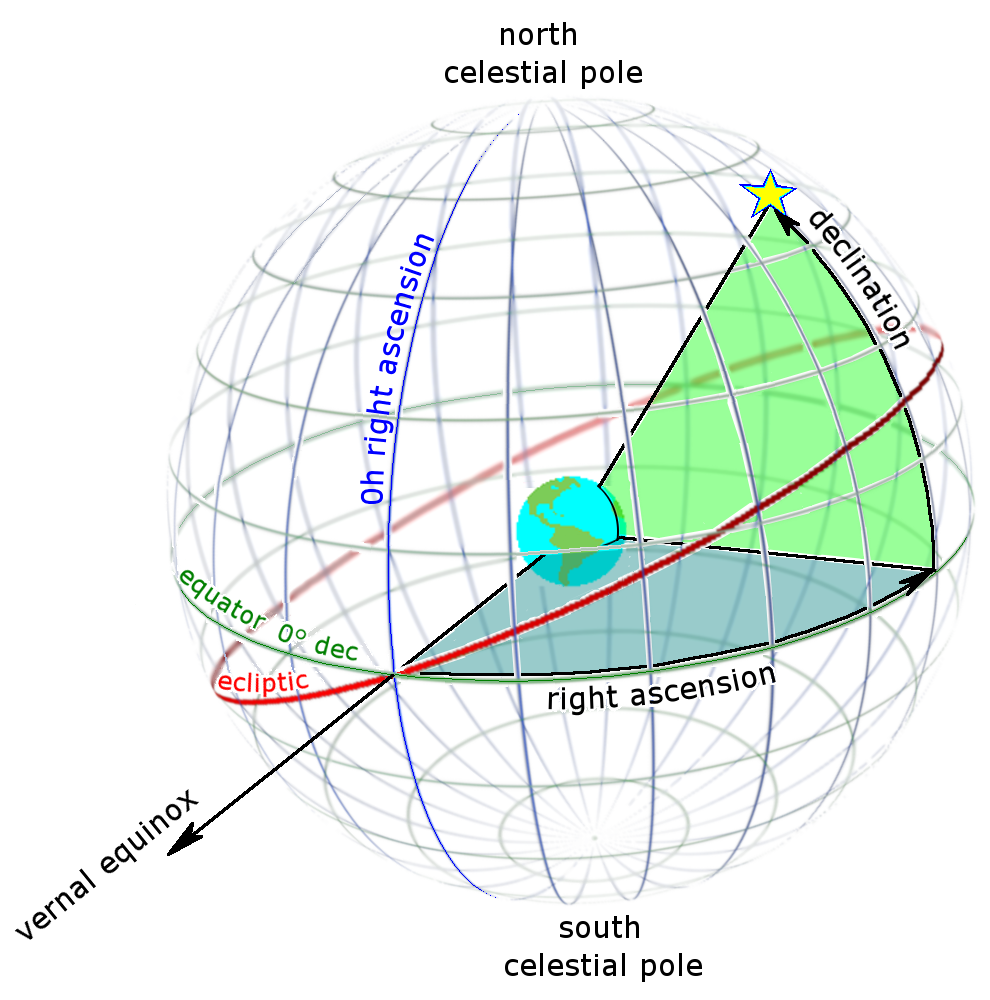
\includegraphics[width=0.55\textwidth]{ARyD.png}
    \caption{Ascensión Recta y Declinación (Créditos 
    Wikipedia)}
\end{figure} 
Esto es especialmente útil cuando no tenemos información de nuestra distancia hasta el cuerpo o solo podemos observarlo con instrumentos que no nos dan esa información. Así pues, usando estos ángulos que sí podemos conocer en función del punto de observación terrestre, podemos obtener una vista preliminar de las órbitas de los objetos celestes que nos interesen.\par

\subsection{Desarrollo del método}

Dado que la deducción matemática no es trivial y para ayudar a la comprensión del lector, explicaremos este método de una forma secuencial e iremos desarrollándolo a modo de algoritmo mientras exponemos las ecuaciones necesarias en cada etapa del mismo.\\

Para comenzar con el método necesitamos partir de algunos datos. Estos son:

\begin{itemize}
    \item Tiempos de observación: $t_1$, $t_2$, $t_3$.
    \item Vectores de posición del observador en dichos tiempos: $\overrightarrow{R_1}$, $\overrightarrow{R_2}$, $\overrightarrow{R_3}$.
            \item Vectores unitarios de dirección topocéntricos: $\hat{\mathbf{\varrho}}_1$, $\hat{\mathbf{\varrho}}_2$, $\hat{\mathbf{\varrho}}_3$. Estos apuntan desde el observador hacia el cuerpo y se pueden obtener antes de empezar midiendo $\alpha$ y $\delta$ del cuerpo en cada tiempo de observación.
\end{itemize}

\begin{figure}[h]
    \centering
    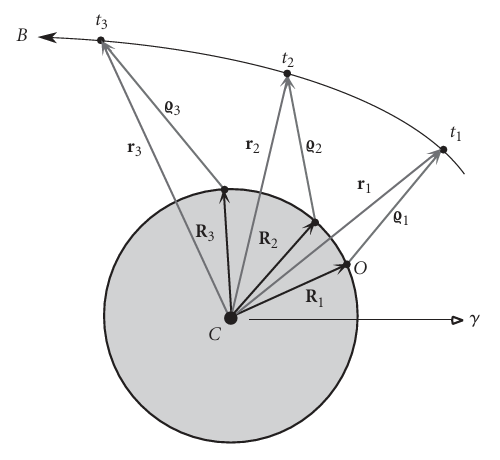
\includegraphics[width=0.65\textwidth]{entra.png}
    \caption{Esquema vectorial de los datos de entrada para el método de Gauss, donde C es el centro de atracción, O el observador y B el cuerpo en órbita. (Créditos 
    HowardD. Curtis)}
\end{figure} 
\newpage
Antes de pasar a ver los pasos, vamos a plantear el problema para ver cómo luego lo resolvemos. Según vemos en la figura 3, los vectores $\overrightarrow{r_i}$ son desconocidos a la vez que necesarios para determinar la órbita del cuerpo. Sin embargo podemos escribir estas tres ecuaciones:\par

\begin{align}
    \overrightarrow{r_1} = \overrightarrow{R_1} + \varrho_1 \hat{\varrho_1} \\
    \overrightarrow{r_2} = \overrightarrow{R_2} + \varrho_2 \hat{\varrho_2} \\
    \overrightarrow{r_3} = \overrightarrow{R_3} + \varrho_3 \hat{\varrho_3}
\end{align}

Al ser ecuaciones vectoriales disponemos de nueve ecuaciones escalares y de 12 incógnitas (las tres componentes de cada vector de posición, más los tres módulos de las direcciones topocéntricas). Como vemos, necesitamos más ecuaciones para poder sacar una solución al sistema.\\

Si seguimos buscando recursos, podemos echar mano de una de las asunciones que hacíamos en el método de Gibbs, en concreto, de que los tres vectores $\overrightarrow{r_i}$ deben pertenecer al mismo plano por la conservación del momento angular (podemos expresar uno de ellos en función de los otros dos). De esto sacamos:

\begin{equation}
    \overrightarrow{r_2} = c_1\cdot\overrightarrow{r_1} + c_3\cdot\overrightarrow{r_3}
\end{equation}

Con esta nueva ecuación vectorial introducimos 2 nuevas incógnitas, los coeficientes $c_1$ y $c_3$. Si hacemos un recuento ahora tenemos 12 ecuaciones para 14 incógnitas. Cada vez estamos más cerca de poder resolver el sistema.\\

Si continuamos buscando ecuaciones que nos ayuden, podemos aprovecharnos de otra consecuencia de la ecuación de movimiento del problema de los dos cuerpos, y es que el vector de estados (que contiene a $\overrightarrow{r}$ y $\overrightarrow{v}$) del cuerpo en órbita se puede expresar como el vector de estados en cualquier tiempo dado mediante los \textbf{coeficientes de Lagrange} de la siguiente forma:

\begin{align}
    \overrightarrow{r_1} = f_1\cdot\overrightarrow{r_2} + g_1\cdot\overrightarrow{v_2} \\
    \overrightarrow{r_3} = f_3\cdot\overrightarrow{r_2} + g_3\cdot\overrightarrow{v_2}
\end{align}

donde $f_i$ y $g_i$ son los coeficientes de Lagrange evaluados en el tiempo $t_i$.\\

Además, si los intervalos de tiempo son lo suficientemente pequeños se puede comprobar que las funciones $f$ y $g$ dependen solo de la distancia al centro de atracción, en nuestro caso, trabajamos con $r_2$. Por tanto, estas dos ecuaciones vectoriales nos añaden 6 ecuaciones escalares y 4 incógnitas (las tres componentes de $\overrightarrow{v_2}$ y la magnitud $r_2$). Si sumamos esto al sistema que ya teníamos, obtenemos un total de 18 ecuaciones escalares para una suma de 18 incógnitas. Por fin el problema está bien preparado para proponer una solución.\\

Antes de empezar, mantengamos en mente que el objetivo será obtener el vector de estados en el instante de tiempo intermedio $t_2$, es decir, $\overrightarrow{r_2}$ y $\overrightarrow{v_2}$, pues con esto determinado podremos obtener los elementos orbitales de la trayectoria de nuestro cuerpo. Visto todo esto, procedamos con los pasos para conseguir nuestro objetivo:\\

\noindent\textbf{1. Obtener intervalos de tiempo}

Primero definimos los intervalos de tiempo $\tau_1$, $\tau_3$ y $\tau$ de la siguiente forma:

\begin{align}
    \tau_1= t_1-t_2 \\
    \tau_3= t_3-t_2 \\
    \tau= \tau_3-\tau_1
\end{align}

Estos son los intervalos de tiempo entre las observaciones y el intervalo de tiempo total. Como explicamos antes, si los intervalos son suficientemente cortos, podremos aprovechar las propiedades de los coeficientes de Lagrange.\\

\newpage
\noindent\textbf{2. Obtener productos vectoriales $p_i$}

Para poder resolver el sistema de ecuaciones necesitaremos calcular los siguientes productos vectoriales para posteriormente simplificar los productos escalares triples.
\begin{align}
    \overrightarrow{p_1}=\hat{\varrho_2}\times\hat{\varrho_3} \hspace{1.5cm} & \overrightarrow{p_2}=\hat{\varrho_1}\times\hat{\varrho_3} \hspace{1cm} & \overrightarrow{p_3}=\hat{\varrho_1}\times\hat{\varrho_3}
\end{align}

\noindent\textbf{3. Obtener productos escalares triples $D$}

Haciendo uso de los productos vectoriales calculados anteriormente, vamos a calcular las siguientes cantidades escalares:

\begin{equation}
    D_0=\hat{\varrho_1}\cdot\overrightarrow{p_1}
\end{equation}

\begin{equation}
\begin{array}{ccc}
D_{11} = \overrightarrow{R_1} \cdot \overrightarrow{p_1} & D_{12} = \overrightarrow{R_1} \cdot \overrightarrow{p_2} & D_{13} = \overrightarrow{R_1} \cdot \overrightarrow{p_3} \\
D_{21} = \overrightarrow{R_2} \cdot \overrightarrow{p_1} & D_{22} = \overrightarrow{R_2} \cdot \overrightarrow{p_2} & D_{23} = \overrightarrow{R_2} \cdot \overrightarrow{p_3} \\
D_{31} = \overrightarrow{R_3} \cdot \overrightarrow{p_1} & D_{32} = \overrightarrow{R_3} \cdot \overrightarrow{p_2} & D_{33} = \overrightarrow{R_3} \cdot \overrightarrow{p_3}
\end{array}
\end{equation}

Estas magnitudes son necesarias ya que en el desarrollo del sistema, nos vamos a topar con expresiones para los $\varrho_i$ y el resto de incógnitas en función de estos productos. Tenerlos calculados nos permite agilizar el proceso.\\

\noindent\textbf{4. Obtener expresiones para las longitudes $\varrho_i$}

Este paso precisa de haber hecho un desarrollo de nuestras ecuaciones del sistema empleando cálculo vectorial. Para evitar atascarnos despejando ecuaciones, vamos a mostrar el procedimiento y sus resultados, dejando como tarea pendiente demostrar las ecuaciones que vamos a presentar.\\

Partiremos de la ecuación 3.4 resolviendo para $c_1$ y $c_3$:

\begin{equation}
    c_1 = \frac{(\overrightarrow{r_2} \times \overrightarrow{r_3}) \cdot (\overrightarrow{r_1} \times \overrightarrow{r_3})}{\|\overrightarrow{r_1} \times \overrightarrow{r_3}\|^2}
\end{equation}

\begin{equation}
    c_3 = \frac{(\overrightarrow{r_2} \times \overrightarrow{r_1}) \cdot (\overrightarrow{r_3} \times \overrightarrow{r_1})}{\|\overrightarrow{r_1} \times \overrightarrow{r_3}\|^2}
\end{equation}

Si ahora utilizamos las ecuaciones 3.5 y 3.6, que expresan $\overrightarrow{r_1}$ y $\overrightarrow{r_3}$ en función de los coeficientes de Lagrange, entonces podemos sustituir en estas ecuaciones para $c_1$ y $c_3$, obteniendo:
\begin{equation}
c_1 = \frac{g_3}{f_{1}g_3 - f_{3}g_1}
\end{equation}

\begin{equation}
c_3 = -\frac{g_1}{f_{1}g_3 - f_{3}g_1}
\end{equation}

Hemos conseguido expresarlos solo en función de estos coeficientes de Lagrange que podemos calcular ahora. 
\newpage
Como hemos asumido que nuestros intervalos de tiempos son lo suficientemente cortos, entonces las expresiones para $f_i$ y $g_i$ toman la siguiente forma:

\begin{equation}
\begin{array}{cc}
f_1 \approx 1 - \frac{1}{2} \frac{\mu}{r_2^3} \tau_1^2 & g_1 \approx \tau_1 - \frac{1}{6} \frac{\mu}{r_2^3} \tau_1^3 \\[1.5em]
f_3 \approx 1 - \frac{1}{2} \frac{\mu}{r_2^3} \tau_3^2 & g_3 \approx \tau_3 - \frac{1}{6} \frac{\mu}{r_2^3} \tau_3^3
\end{array}
\end{equation}

Donde recordamos $\mu$ es el parámetro gravitacional. Estas ecuaciones nos permiten ahora conocer el denominador de las ecuaciones 3.15 y 3.16 para continuar con la manipulación de esas expresiones. Esto es:

\begin{align}
    f_{13} - f_{31} &= \left( 1 - \frac{1}{2} \frac{\mu}{r_2^3} \tau_1^2 \right) 
    \left( \tau_3 - \frac{1}{6} \frac{\mu}{r_2^3} \tau_3^3 \right) - \left( 1 - \frac{1}{2} \frac{\mu}{r_2^3} \tau_3^2 \right) 
    \left( \tau_1 - \frac{1}{6} \frac{\mu}{r_2^3} \tau_1^3 \right) \notag\\
    &= (\tau_3 - \tau_1) - \frac{1}{6} \frac{\mu}{r_2^3} (\tau_3 - \tau_1)^3  + \frac{1}{12} \frac{\mu^2}{r_2^6} (\tau_1^2 \tau_3^3 - \tau_1^3 \tau_3^2) \notag\\
    &\approx \tau - \frac{1}{6} \frac{\mu}{r_2^3} \tau^3
\end{align}

donde lo que hacemos en la última aproximación es quedarnos con los términos más significativos. Si ahora introducimos este resultado en la ecuación 3.15 obtenemos:

\begin{equation}
    c_1 \approx \frac{\tau_3 - \frac{1}{6} \frac{\mu}{r_2^3} \tau_3^3}{\tau - \frac{1}{6} \frac{\mu}{r_2^3} \tau^3} 
    = \frac{\tau_3}{\tau} \left( 1 - \frac{1}{6} \frac{\mu}{r_2^3} \tau_3^2 \right) \cdot \left( 1 - \frac{1}{6} \frac{\mu}{r_2^3} \tau^2 \right)^{-1}
\end{equation}

Que podemos simplificar aún más manipulando el último término de la derecha para obtener:

\begin{equation}
c_1 \approx \frac{\tau_3}{\tau} \left[ 1 + \frac{1}{6} \frac{\mu}{r_2^3} (\tau^2 - \tau_3^2) \right]
\end{equation}

Haciendo lo propio para el otro coeficiente:

\begin{equation}
c_3 \approx -\frac{\tau_1}{\tau} \left[ 1 + \frac{1}{6} \frac{\mu}{r_2^3} (\tau^2 - \tau_1^2) \right]
\end{equation}

Hemos logrado expresar estos valores en términos de los intervalos temporales y de la distancia desconocida $r_2$ al centro de atracción, lo que nos permite ahora buscar expresiones para $\varrho_1$, $\varrho_2$ y $\varrho_3$ en función de los coeficientes $c_1$ y $c_2$.\\

Para realizar esto, vamos a sustituir las ecuaciones 3.1, 3.2 y 3.3 en la ecuación 3.4 para conseguir una ecuación de donde poder despejar cada $\varrho$. Vamos a tener una sola ecuación para las tres, pero podemos manipularla de forma ingeniosa para quedarnos solo con una de ellas a la vez. Esto lo haremos multiplicando la ecuación por el producto vectorial adecuado. Tras estudiar exhaustivamente cada caso, nos vamos a dar cuenta de que los cálculos resultantes estarán escritos en función de las magnitudes y productos que ya tenemos calculados de apartados anteriores, esto es, todas las $D$'s del paso 3.\\

Como hemos dicho, si resolvemos para cada distancia $\varrho$ y asumimos que $\mbox{$D_0 \neq 0$}$ (lo que implica que $\hat{\varrho_1}$, $\hat{\varrho_2}$ y $\hat{\varrho_3}$ no están en el mismo plano), las expresiones que nos quedan son las siguientes:

\begin{equation}
\varrho_1 = \frac{1}{D_0} \left( -D_{11} + \frac{1}{c_1} D_{21} - \frac{c_3}{c_1} D_{31} \right)
\end{equation}

\begin{equation}
\varrho_2 = \frac{1}{D_0} (-c_1 D_{12} + D_{22} - c_3 D_{32})
\end{equation}

\begin{equation}
\varrho_3 = \frac{1}{D_0} \left( -\frac{c_1}{c_3} D_{13} + \frac{1}{c_3} D_{23} - D_{33} \right)
\end{equation}

Si ahora sustituimos las expresiones que habíamos encontrado para $c_1$ y $c_2$ (ecuaciones 3.20 y 3.21) en estas, obtenemos nuestros resultados finales para este paso:

\begin{equation}
    \varrho_2 = A + \frac{\mu B}{r_2^3}
\end{equation}

donde:
\begin{equation}
A = \frac{1}{D_0} \left( -D_{12} \frac{\tau_3}{\tau} + D_{22} + D_{32} \frac{\tau_1}{\tau} \right)
\end{equation}

\begin{equation}
B = \frac{1}{6D_0} \left[ D_{12} (\tau_3^2 - \tau^2) \frac{\tau_3}{\tau} + D_{32} (\tau^2 - \tau_1^2) \frac{\tau_1}{\tau} \right]
\end{equation}

y las otras dos distancias:
\begin{equation}
\varrho_1 = \frac{1}{D_0} \left[ \frac{6 \left( D_{31} \frac{\tau_1}{\tau_3} + D_{21} - \frac{\tau}{\tau_3} \right) r_2^3 + \mu D_{31} (\tau^2 - \tau_1^2) \frac{\tau_1}{\tau_3}}{6r_2^3 + \mu (\tau^2 - \tau_3^2)} - D_{11} \right]
\end{equation}

\begin{equation}
\varrho_3 = \frac{1}{D_0} \left[ \frac{6 \left( D_{13} \frac{\tau_3}{\tau_1} - D_{23} - \frac{\tau}{\tau_1} \right) r_2^3 + \mu D_{13} (\tau^2 - \tau_3^2) \frac{\tau_3}{\tau_1}}{6r_2^3 + \mu (\tau^2 - \tau_3^2)} - D_{33} \right]
\end{equation}

La ecuación 3.25 establece una relación entre la distancia topocéntrica entre el cuerpo y el observador $\varrho_2$ y la distancia geocéntrica al centro de atracción $r_2$. Esto, si pensamos en el objetivo final, es muy potente pues con determinar un valor válido de $r_2$, podremos sustituir en estas ecuaciones y con los rangos $\varrho_i$ calculados podremos sustituir en las ecuaciones 3.1, 3.2 y 3.3 para obtener las posiciones del cuerpo en los instantes de tiempo correspondientes.
\newpage
\noindent\textbf{5. Obtener valor de $r_2$ y de $\overrightarrow{r_2}$}

Como acabamos de explicar, vamos a buscar este valor para poder cerrar el proceso de búsqueda de los vectores de posición. Por tanto, vamos a coger la ecuación 3.2 y vamos a multiplicar sus términos por $\overrightarrow{r_2}$ para obtener lo siguiente:

\begin{equation}
r_2^2 = \varrho_2^2 + 2E \varrho_2 + R_2^2
\end{equation}

donde $E=\overrightarrow{R_{2}}\cdot\hat{\varrho_{2}}$. Si ahora cogemos y sustituimos la ecuación 3.25 en esta última, obtenemos: 

\begin{equation}
    r_2^2 = \left( A + \frac{\mu B}{r_2^3} \right)^2 + 2E \left( A + \frac{\mu B}{r_2^3} \right) + R_2^2
\end{equation}

Si desarrollamos esta ecuación y la expandimos, resulta en un polinomio de grado 8 de la siguiente forma: 

\begin{equation}
    r_2^8 + ar_2^6 + br_2^3 + c = 0
\end{equation}

donde los valores de los coeficientes son:

\begin{equation*}
    a = -(A^2 + 2AE + R_2^2) \quad b = -2\mu B(A + E) \quad c = -\mu^2 B^2
\end{equation*}

Podemos obtener numéricamente las raíces de este polinomio y por tanto encontrar un valor adecuado para $r_2$. Una vez encontrado, podemos sustituirlo en la ecuación 3.25 para hallar el valor de $\varrho_2$ e introducir este último en la ecuación 3.2 para hallar finalmente el vector de posición en el tiempo intermedio, $\overrightarrow{r_2}$. Acabamos de lograr la primera parte de nuestro objetivo.\\

\noindent\textbf{6. Obtener valor de $\overrightarrow{v_2}$}

Para terminar, primero recordamos que a pesar de que estemos resolviendo para $\overrightarrow{r_2}$, los valores $\overrightarrow{r_1}$ y $\overrightarrow{r_3}$ también son calculables en este punto y, de hecho, los necesitamos para poder concluir en este paso. Vamos a partir de la ecuación 3.5, de la cual vamos a despejar $\overrightarrow{r_2}$:

\begin{equation}
    \overrightarrow{r_2} = \frac{1}{f_1} \overrightarrow{r_1} - \frac{g_1}{f_1} \overrightarrow{v_2} 
\end{equation}

Vemos que aparecen los coeficientes de Lagrange que teníamos anteriormente. La diferencia es que ahora podemos calcularlos analíticamente pues ya disponemos del valor de $r_2$. Si ahora sustituimos esta ecuación para $\overrightarrow{r_2}$ en la ecuación 3.6:

\begin{equation}
    \overrightarrow{r_3} = \frac{f_3}{f_1} \overrightarrow{r_1} + \left( \frac{f_1 g_3 - f_3 g_1}{f_1} \right) \overrightarrow{v_2}
\end{equation}

Y por último, si despejamos y resolvemos para $\overrightarrow{v_2}$ nos queda:

\begin{equation}
    \overrightarrow{v_2} = \frac{1}{f_1 g_3 - f_3 g_1} (-f_3 \overrightarrow{r_1} + f_1 \overrightarrow{r_3})
\end{equation}

Con esto acabamos de completar nuestro objetivo, hemos obtenido el vector $\overrightarrow{v_2}$ y por tanto completado nuestro vector de estados (ya habíamos obtenido $\overrightarrow{r_2}$ en el paso anterior). Con este, podemos calcular los elementos orbitales del cuerpo y por tanto determinar un modelo preliminar de su órbita.\\

\noindent\textbf{7. Iterar y corregir}

El método de Gauss no termina ahí. Los valores $\overrightarrow{v_2}$ y $\overrightarrow{r_2}$ son valores aproximados que hay que iterar hasta que consigan el nivel de tolerancia o convergencia requerido por el usuario. Con un algoritmo complementario al que se sigue para llegar hasta aquí, se pueden perfeccionar estos valores que comentamos para calcular con mayor precisión los coeficientes de Lagrange (intentamos conseguir sus valores "exactos"), y con ellos volver a calcular todos los parámetros que habíamos implementado. Habrá parámetros como las distancias $\varrho_i$ que no cambien una vez hecha esta primera mejora, pero el valor del vector de estados será más preciso. Con este nuevo valor se pueden volver a calcular las funciones $f$ y $g$ (Lagrange) y repetir todo este proceso para obtener un $\overrightarrow{v_2}$ y $\overrightarrow{r_2}$ más exactos aún. La precisión con la que se detendrá el cálculo es decisión de la persona que lo implemente.\\

Vemos que el hecho de que el método de Gauss sea un proceso iterativo proporciona muchísima más precisión y por tanto que sea uno de los más elegidos en la determinación preliminar de órbitas en las que se quiere mantener una buena fiabilidad.
\section{Resultados} 
\index{Resultados} 
En esta sección mostraremos los resultados obtenidos tras haber 
implementado ambos métodos en MATLAB. Cabe destacar que para obtener los datos de partida para ambos métodos se ha hecho uso de software externo. Al ser herramientas potentes y con bastante peso en el trabajo, hemos recogido la información pertinente en el Anexo I.\\

\subsection{Método de Gibbs}
Para el empleo del método de Gibbs hemos decidido hacer 
una determinación de manera preliminar de la órbita del 
planeta Mercurio y comparar los resultados obtenidos con los 
valores reales (aunque la parte del análisis se hará en 
la siguiente sección). \\

Como sabemos, el método de Gibbs necesita de 3 posiciones 
del cuerpo en la órbita. Es por ello que para obtener estas 
posiciones se ha hecho uso de 2 herramientas que pueden ser consultadas en el Anexo correspondiente. \\

Habiendo obtenido de las mismas el módulo de la distancia de Mercurio al Sol, los días correspondientes a las observaciones y la latitud y longitud heliocéntricas, entonces podemos obtener las componentes de nuestros vectores posición de la siguiente manera:

\begin{align*}
    &r_{x}=r\cos(\beta)\cos(\lambda) \\
    &r_{y}=r\cos(\beta)\sin(\lambda) \\
    &r_{z}=r\sin(\beta)
\end{align*}

Siendo $r$ el módulo obtenido previamente con la primera herramienta; 
$\beta$ la latitud heliocéntrica y $\lambda$ la longitud heliocéntrica. \\

Con todo esto, ya estamos en disposición de mostrar 
los resultados obtenidos. Cabe recalcar que se han obtenido resultados 
para cada vector de posición. Estos resultados para $\overrightarrow{r_{1}}$ han sido: 

\begin{center}
    \centering
    \begin{tabular}{|c|c|c|}
    \hline
    $\overrightarrow{r}\, (km)$ & $\overrightarrow{v}\, (km/s)$ & $h\, ( km^{2}/s)$  \\ \hline
    $(-3.46,3.59,0.61)\cdot10^7$ & $(-43.37, -30.07, 2.22)$ & $2,62 \cdot 10^{9}$\\ \hline
    \end{tabular}
\end{center}

\begin{center}
    \centering
    \begin{tabular}{|c|c|c|c|c|c|c|c|}
    \hline
     $i\, (^{\circ})$ & $\Omega\, (^\circ)$ & $e$ & $\omega\, (^\circ)$ & $a\, (km)$ & $\theta (^\circ)$ & $r_{p}\, (km)$ & $T\, (dias)$\\ \hline
    $7.10$ & $54.46$ & $0.17$ & $358.37$ & $5.32\cdot 10^{7}$ & $81.17$ & $4.40\cdot 10^{7}$ & $77.31$ \\ \hline
    \end{tabular}
\end{center}
Por su parte, para $\overrightarrow{r_{2}}$ obtuvimos:

\begin{center}
    \centering
    \begin{tabular}{|c|c|c|}
    \hline
    $\overrightarrow{r}\, (km)$ & $\overrightarrow{v}\, (km/s)$ & $h\, ( km^{2}/s)$  \\ \hline
    $(-4.51,2.65,0.63)\cdot10^7$ & $(-32.91, -38.31, -0.78)$ & $2,62 \cdot 10^{9}$\\ \hline
    \end{tabular}
\end{center}

\begin{center}
    \centering
    \begin{tabular}{|c|c|c|c|c|c|c|c|}
    \hline
     $i\, (^{\circ})$ & $\Omega\, (^\circ)$ & $e$ & $\omega\, (^\circ)$ & $a\, (km)$ & $\theta (^\circ)$ & $r_{p}\, (km)$ & $T\, (dias)$\\ \hline
    $7.19$ & $42.32$ & $0.17$ & $10.41$ & $5.32\cdot 10^{7}$ & $96.72$ & $4.39\cdot 10^{7}$ & $77.41$ \\ \hline
    \end{tabular}
\end{center}
Mientras que para $\overrightarrow{r_{3}}$ obtuvimos:

\begin{center}
    \centering
    \begin{tabular}{|c|c|c|}
    \hline
    $\overrightarrow{r}\, (km)$ & $\overrightarrow{v}\, (km/s)$ & $h\, ( km^{2}/s)$  \\ \hline
    $(-5.27,1.40,0.55)\cdot10^7$ & $(-20.42,-43.00,-3.54)$ & $2.58 \cdot 10^{9}$\\ \hline
    \end{tabular}
\end{center}

\begin{center}
    \centering
    \begin{tabular}{|c|c|c|c|c|c|c|c|}
    \hline
     $i\, (^{\circ})$ & $\Omega\, (^\circ)$ & $e$ & $\omega\, (^\circ)$ & $a\, (km)$ & $\theta (^\circ)$ & $r_{p}\, (km)$ & $T\, (dias)$\\ \hline
    $7.90$ & $32.21$ & $0.18$ & $13.72$ & $5.17\cdot 10^{7}$ & $118.97$ & $4.21\cdot 10^{7}$ & $74.08$ \\ \hline
    \end{tabular}
\end{center}
Como era de esperar, los valores de los elementos orbitales 
que se han obtenido con cada medida son muy similares entre sí, excepto 
en aquellos como $\theta$ en los que su valor depende directamente de 
la posición de nuestro cuerpo celeste. 
El único que difiere un poco de las otras dos es la tercera medida. 
La posible causa de esto junto con un tratamiento de errores 
se hará en la siguiente sección.

\subsection{Método de Gauss}

Para verificar el funcionamiento de este método y su versatilidad, vamos a estudiar dos escenarios. El primero de ellos será determinar la órbita que describe un satélite alrededor de la Tierra y el segundo será determinar de nuevo la órbita de Mercurio alrededor del Sol para poder comparar con los resultados obtenidos con el método de Gibbs.\\

\noindent\textbf{Primer caso: Satélite Meteosat-10.}

En este primer apartado vamos a presentar los resultados obtenidos para la órbita del satélite Meteosat-10 (MSG3). Para empezar, como explicamos en el desarrollo del método, necesitamos tres observaciones del cuerpo en las que tomemos datos de la ascensión recta y de la declinación. Además, adicionalmente y para poder hacer el cálculo vectorial correcto, precisamos de la latitud del puesto de observación y del tiempo local sidéreo. Estos dos ángulos son necesarios para ubicarnos correctamente sobre la superficie terrestre y para proporcionarle los vectores correctos a la entrada de nuestro método.\\

Los datos iniciales han sido recogidos de la misma fuente que para el método anterior. Recordamos que en este método se obtiene un único vector de estados correspondiente a la observación intermedia. Con todo esto, los resultados obtenidos han sido:

\begin{center}
    \centering
    \begin{tabular}{|c|c|c|}
    \hline
    $\overrightarrow{r}\, (km)$ & $\overrightarrow{v}\, (km/s)$ & $h\, ( km^{2}/s)$  \\ \hline
    $(4.59, 0.30, -0.18)\cdot10^4$ & $(-0.14, 3.00, 0.07)$ & $1.39 \cdot 10^{5}$\\ \hline
    \end{tabular}
\end{center}

\begin{center}
    \centering
    \begin{tabular}{|c|c|c|c|c|c|c|c|}
    \hline
     $i\, (^{\circ})$ & $\Omega\, (^\circ)$ & $e$ & $\omega\, (^\circ)$ & $a\, (km)$ & $\theta (^\circ)$ & $r_{p}\, (km)$ & $T\, (dias)$\\ \hline
    $2.71$ & $61.47$ & $ 0.048$ & $281.90$ & $4.83\cdot 10^{4}$ & $20.39$ & $4.59\cdot 10^{4}$ & $1.22$ \\ \hline
    \end{tabular}
\end{center}


\noindent\textbf{Segundo caso: Mercurio.}

En este caso, para determinar la órbita de Mercurio debemos tomar los datos de las tres observaciones con el sol como origen del sistema de referencia. Afortunadamente, el software encontrado también nos proporciona dicha configuración, así que podemos proceder con la muestra de los resultados. Estos han sido:

\begin{center}
    \centering
    \begin{tabular}{|c|c|c|}
    \hline
    $\overrightarrow{r}\, (km)$ & $\overrightarrow{v}\, (km/s)$ & $h\, ( km^{2}/s)$  \\ \hline
    $(3.71, -2.78, -1.85)\cdot10^7$ & $(41.98, 31.81, 12.83)$ & $2.68 \cdot 10^{9}$\\ \hline
    \end{tabular}
\end{center}

\begin{center}
    \centering
    \begin{tabular}{|c|c|c|c|c|c|c|c|}
    \hline
     $i\, (^{\circ})$ & $\Omega\, (^\circ)$ & $e$ & $\omega\, (^\circ)$ & $a\, (km)$ & $\theta (^\circ)$ & $r_{p}\, (km)$ & $T\, (dias)$\\ \hline
    $28.45$ & $10.44$ & $0.19$ & $242.60$ & $5.58\cdot 10^{7}$ & $66.41$ & $4.51\cdot 10^{7}$ & $83.22$ \\ \hline
    \end{tabular}
\end{center}


\section{Análisis de resultados} %A lo mejor podemos anañizar los resultados aquí
\index{Análisis de resultados}
El objetivo principal de esta sección es comparar los resultados obtenidos con los de la bibliografía y, a partir de eso, sacar las conclusiones pertinentes. Como hemos implementado nuestros métodos con varios ejemplos, vamos a analizar los resultados para cada caso.\par

\subsection{Primer caso: Meteosat-10.}

Los datos que podemos encontrar sobre la órbita del satélite y con los que vamos a comparar los obtenidos son los siguientes:

\begin{center}
    \centering
    \begin{tabular}{|c|c|c|c|c|c|c|}
    \hline
    $\overline{v}\, (km/s)$ & $h\, (km^{2}/s)$ & $i\, (^{\circ})$ & $a\, (km)$ & $e$ & $T\, (dias)$ & $r_{p}\, (km)$\\ \hline
    $3.07$ & $1.32 \cdot 10^{5}$ & $3.4$ & $4.21\cdot 10^{4}$ & $0.00014$ & $0.997$ & $4.21\cdot10^4$\\ \hline
    \end{tabular}
\end{center}

Los datos angulares, al variar con la posición, los dejamos excluidos de este apartado. Como este caso solo lo hemos estudiado con el método de Gauss, vamos a estudiar las discrepancias entre estos valores teóricos y los que hemos obtenido al aplicar dicho método.

\subsubsection{Velocidad}

Comenzaremos por calcular el módulo de la velocidad que hemos obtenido:

\begin{equation*}
    v=\sqrt{(-0.14)^2+(3)^2+(0.07)^2}\approx3.004 km/s
\end{equation*}

Y ahora veremos su error relativo:

\begin{equation*}
    \epsilon=\frac{\left\lvert \overline{v}-\overline{v}_{exp} \right\rvert }{\overline{v}}=0.0214=2.14\%
\end{equation*}

Vemos que en este primer aspecto hemos logrado hacer una buena aproximación.

\subsubsection{Momento angular específico}
Procedemos de manera análoga para esta magnitud:

\begin{equation*}
    \epsilon=\frac{\left\lvert h-h_{exp} \right\rvert}{h}=0.0530=5.3\%
\end{equation*}

Consiguiendo un valor aceptable.

\subsubsection{Inclinación}
Procedemos de manera análoga para esta magnitud:

\begin{equation*}
    \epsilon=\frac{\left\lvert i-i_{exp} \right\rvert}{i}=0.2029=20.29\%
\end{equation*}

Este error sí que es considerable. El valor elevado del error es atribuible a que son medidas muy pequeñas que deberían ser medidas con mucha más precisión. 

\subsubsection{Semieje mayor}
Procedemos de manera análoga para esta magnitud:

\begin{equation*}
    \epsilon=\frac{\left\lvert a-a_{exp} \right\rvert}{a}=0.1472=14.72\%
\end{equation*}

De nuevo, una discrepancia significativa en nuestros resultados.

\subsubsection{Excentricidad}
Procedemos de manera análoga para esta magnitud:

\begin{equation*}
    \epsilon=\frac{\left\lvert e-e_{exp} \right\rvert}{e}=341.85\approx30000\%
\end{equation*}

Aquí nos encontramos con un error enorme en la predicción de la órbita. Aún así, no debemos dejarnos llevar por la magnitud del error, ya que vamos a intentar buscar una explicación para el mismo. La principal razón es la excentricidad tan baja que tiene este satélite. Un valor tan próximo a cero hace que las predicciones numéricas se vuelvan complicadas y hace que cualquier pequeña desviación se represente como un error relativo elevado.\\

Con esto, creemos que el error relativo no es una buena manera de medir nuestras discrepancias en este caso. Nuestro resultado, que recordamos es $e=0.048$, sigue siendo lo suficientemente bajo como para interpretar que la órbita es cercana a una circunferencia. Con esto, podemos representar dos órbitas genéricas con los dos valores de excentricidad para comprobar que, como decimos, la diferencia no es tan exagerada como muestra este error.

\begin{figure}[h]
    \centering
    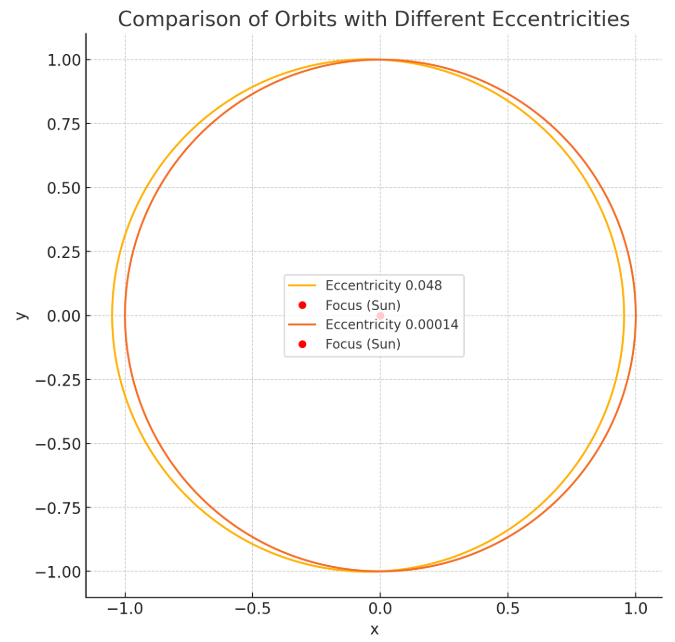
\includegraphics[width=0.5\linewidth]{exce.png}
    \caption{Comparación excentricidades en órbitas casi circulares.}
\end{figure}

\subsubsection{Periodo}
Procedemos de manera análoga para esta magnitud:

\begin{equation*}
    \epsilon=\frac{\left\lvert T-T_{exp} \right\rvert}{T}=0.2236=22.36\%
\end{equation*}

El periodo de los satélites geoestacionarios como este debería coincidir con la duración de un día terrestre. Como hemos visto, nos sale un valor ligeramente superior que hace que aparezca este error.

\subsubsection{Radio del periastro}

\begin{equation*}
    \epsilon=\frac{\left\lvert r_p-r_{p,\,exp} \right\rvert}{T}=0.0902=9.02\%
\end{equation*}

Al ser una órbita casi circular, el error es aproximadamente del mismo orden que el del semieje mayor.

\subsection{Segundo caso: Mercurio}
Comenzamos de nuevo mostrando los valores de los elementos orbitales 
de la órbita de Mercurio de la literatura: 

\begin{center}
    \centering
    \begin{tabular}{|c|c|c|c|c|c|c|}
    \hline
    $\overline{v}\, (km/s)$ & $h\, (km^{2}/s)$ & $i\, (^{\circ})$ & $a\, (km)$ & $e$ & $T\, (dias)$ & $r_{p}\, (km)$\\ \hline
    $47,87$ & $2,71 \cdot 10^{9}$ & $7,005$ & $5,791\cdot 10^{7}$ & $0,2056$ & $87,97$ & $4.604\cdot10^7$\\ \hline
    \end{tabular}
\end{center}

Con estos datos en cuenta podemos comenzar nuestro análisis. Este caso ha sido estudiado por los dos métodos de forma premeditada para poder comparar la eficacia de ambos métodos para un mismo escenario. Así pues, iremos elemento a elemento comparando los errores obtenidos para cada procedimiento.

\subsubsection{Velocidad}
\noindent\textbf{Método de Gibbs}\par
Para comparar las velocidades, lo primero de todo vamos a 
calcular el módulo de las 3 velocidades que hemos obtenido: 
\begin{align*}
    &v_{1}=52,82\, km/s \\
    &v_{2}=50,51\, km/s  \\
    &v_{3}=47,73\, km/s 
\end{align*}
Como podemos ver, según lo que nos indica la velocidad media 
de la literatura, nuestros 3 valores entran dentro de lo esperado. 
Para calcular el error cometido, ya que el dato que la literatura 
nos proporciona es una velocidad media, vamos a calcular la 
velocidad media de nuestras tres medidas y calcular el error 
relativo. 
\begin{equation*}
    \overline{v}_{exp}=\frac{v_{1}+v_{2}+v_{3}}{3}=50,35  
\end{equation*}
El error cometido es de 
\begin{equation*}
    \epsilon=\frac{\left\lvert \overline{v}-\overline{v}_{exp} \right\rvert }{\overline{v}}=0,052=5,2\%
\end{equation*}
Como vemos, hemos cometido un error bastante pequeño y que entra 
dentro de nuestros márgenes aceptables.\\

\noindent\textbf{Método de Gauss}\par
Haciendo lo propio con lo obtenido en este método:

\begin{equation*}
    v=\sqrt{(41.98)^2+(31.81)^2+(12.83)^2}\approx54.21 km/s
\end{equation*}

\begin{equation*}
    \epsilon=\frac{\left\lvert \overline{v}-\overline{v}_{exp} \right\rvert }{\overline{v}}=0.1324=13.24\%
\end{equation*}

Obteniendo en este caso un valor de error más elevado que con el otro método.

\subsubsection{Momento angular específico}
\noindent\textbf{Método de Gibbs}\par
A partir de la determinación de este error, lo que vamos a 
hacer va a ser comparar el error para cada medida obtenida. \\

Comenzando con el valor obtenido de la primera posición tenemos 
un error de 
\begin{align*}
    &\epsilon_{1}=\frac{\left\lvert h-h_{exp1} \right\rvert }{h}=0,033=3,3\% \\
    &\epsilon_{2}=\frac{\left\lvert h-h_{exp2} \right\rvert }{h}=0,033=3,3\% \\
    &\epsilon_{3}=\frac{\left\lvert h-h_{exp3} \right\rvert }{h}=0,047=4,8\% \\
\end{align*}
Todos los errores que hemos obtenido son inferiores al $5\%$ 
validando una vez más el método de Gibbs.\\

\noindent\textbf{Método de Gauss}\par
Si procedemos para el método de Gauss:

\begin{equation*}
    \epsilon=\frac{\left\lvert h-h_{exp} \right\rvert}{h}=0.011=1.1\%
\end{equation*}

Obteniendo una buena medida para esta magnitud.

\subsubsection{Inclinación}
\noindent\textbf{Método de Gibbs}\par
Para la inclinación hemos cometido un error de 
\begin{align*}
    &\epsilon_{1}=\frac{\left\lvert i-i_{exp1} \right\rvert }{i}=0,014=1,4\% \\
    &\epsilon_{2}=\frac{\left\lvert i-i_{exp2} \right\rvert }{i}=0,036=2,6\% \\
    &\epsilon_{3}=\frac{\left\lvert i-i_{exp3} \right\rvert }{i}=0,127=12,7\% \\
\end{align*}
En este caso, vemos que el error para el valor de $r_{3}$ empieza 
a ser un poco elevado. La hipótesis principal que barajamos 
sobre por qué sucede esto es que, al ser un valor de la inclinación 
tan bajo, para obtener un error aceptable nuestras medidas deben 
ser muy precisas y en el caso de la tercera, a pesar de cometer 
un error absoluto de solo $0,9$ aproximadamente, parece no 
ser lo suficientemente preciso.\\

\noindent\textbf{Método de Gauss}\par
Si procedemos para el método de Gauss:

\begin{equation*}
    \epsilon=\frac{\left\lvert i-i_{exp} \right\rvert}{i}=3.06\approx300\%
\end{equation*}

Como podemos apreciar, esta vez es el valor de la inclinación el que se nos dispara a pesar de que el resto de elementos orbitales encajen con la órbita de Mercurio. Aún así, aunque la discrepancia es grande, el valor del error no se ve tan incrementado como en el caso de la excentricidad del escenario anterior.\\

Queremos destacar en este punto la premisa de que estos son métodos preliminares. Tanto el método de Gibbs como el de Gauss descritos trabajan con la dinámica de dos cuerpos. Un valor de inclinación tan dispar del valor real nos podría llevar a concluir que hemos determinado la órbita de otro cuerpo. Sin embargo, en la realidad te enfrentas a estas incertidumbres con métodos que tienen en cuenta sistemas dinámicos más complejos, así como de tres o más cuerpos.\\

Si la órbita de Mercurio no fuera conocida y esta fuera la primera vez que se estudia, con total seguridad verificar los resultados con otros métodos nos llevaría a la conclusión de que este valor para la inclinación es imposible. En resumen, la obtención de valores erróneos en métodos preliminares no es improbable, y validación de resultados requiere de métodos más sofisticados que respalden o contradigan tus hipótesis obtenidas por los primeros.\\

\subsubsection{Semieje mayor}
\noindent\textbf{Método de Gibbs}\par
Para el semieje mayor hemos cometido unos errores de 
\begin{align*}
    &\epsilon_{1}=\frac{\left\lvert a-a_{exp1} \right\rvert }{a}=0,081=8,1\% \\
    &\epsilon_{2}=\frac{\left\lvert a-a_{exp2} \right\rvert }{a}=0,081=8,1\% \\
    &\epsilon_{3}=\frac{\left\lvert a-a_{exp3} \right\rvert }{a}=0,107=10,7\% \\
\end{align*}
De nuevo, el error para $r_{3}$ es un poco alto y en este caso, similar a lo que sucedía en el anterior, el error elevado que 
obtenemos es debido a que los órdenes de magnitud tan grandes 
que estamos manejando para el semieje que, de nuevo, nos 
demandan más precisión.\\

\noindent\textbf{Método de Gauss}\par

\begin{equation*}
    \epsilon=\frac{\left\lvert a-a_{exp} \right\rvert}{a}=0.036=3.6\%
\end{equation*}

Consiguiendo un buen valor aproximado.

\subsubsection{Excentricidad}
\noindent\textbf{Método de Gibbs}\par
Los errores que obtenemos en la excentricidad son 
\begin{align*}
    &\epsilon_{1}=\frac{\left\lvert e-e_{exp1} \right\rvert }{e}=0,173=17,3\% \\
    &\epsilon_{2}=\frac{\left\lvert a-a_{exp2} \right\rvert }{e}=0,173=17,3\% \\
    &\epsilon_{3}=\frac{\left\lvert e-e_{exp3} \right\rvert }{e}=0,125=12,5\% \\
\end{align*}
En este caso, todos los errores cometidos son altos y la 
razón es la misma que para la inclinación. La diferencia 
tan grande de error entre las medidas de $r_{1}$ y $r_{2}$ 
respecto a $r_{3}$ (de casi un $5\%$ de diferencia) nos da 
indicios de que nuestras suposiciones de la razón de los 
valores altos de error a pesar de que los datos obtenidos 
son cercanos a los de la literatura es cierta.\\

\noindent\textbf{Método de Gauss}\par

\begin{equation*}
    \epsilon=\frac{\left\lvert e-e_{exp} \right\rvert}{e}=0.075=7.5\%
\end{equation*}

Obtenemos un mejor valor para la excentricidad que, desde luego, en el primer escenario. Esto puede ser debido a que esta órbita no tiene una excentricidad tan cercana a cero, es decir, difiere más de una circunferencia.

\subsubsection{Periodo}
\noindent\textbf{Método de Gibbs}\par
Para el periodo los errores son de:
\begin{align*}
    &\epsilon_{1}=\frac{\left\lvert T-T_{exp1} \right\rvert }{T}=0,121=12,1\% \\
    &\epsilon_{2}=\frac{\left\lvert T-T_{exp2} \right\rvert }{T}=0,120=12,0\% \\
    &\epsilon_{3}=\frac{\left\lvert T-T_{exp3} \right\rvert }{T}=0,157=15,7\% \\
\end{align*}
En este caso, hay una razón en específico que hace que los 
errores en los periodos sean elevados. Esto es debido a que 
la fórmula empleada para calcular el periodo es 
\begin{equation*}
    T=2\pi\sqrt{\frac{a^{3}}{\mu}}
\end{equation*}
Como vemos, para calcular el periodo se emplea el semieje mayor. 
Como esta medida ya tiene un error asociado de por sí, el 
periodo también va a tener un error propiciado por el 
semieje y esto hace que el error cometido en el cálculo 
se incremente significativamente.\\

\noindent\textbf{Método de Gauss}\par

\begin{equation*}
    \epsilon=\frac{\left\lvert T-T_{exp} \right\rvert}{T}=0.0539=5.4\%
\end{equation*}

En este método obtenemos una mejor aproximación para el valor del periodo.

\subsubsection{Radio del periastro}
\noindent\textbf{Método de Gibbs}\par
Los errores que obtenemos en la excentricidad son 
\begin{align*}
    &\epsilon_{1}=\frac{\left\lvert r_p-r_{p,exp1} \right\rvert }{r_p}=0.0443=4.4\% \\
    &\epsilon_{2}=\frac{\left\lvert r_p-r_{p,exp2} \right\rvert }{r_p}=0.0464=4.6\% \\
    &\epsilon_{3}=\frac{\left\lvert r_p-r_{p,exp3} \right\rvert }{r_p}=0.0855=8.5\% \\
\end{align*}

Como vemos, conseguimos valores aceptables para este elemento.\\

\noindent\textbf{Método de Gauss}\par

\begin{equation*}
    \epsilon=\frac{\left\lvert r_p-r_{p,exp} \right\rvert }{r_p}=0.0204=2.04\%
\end{equation*}

Y con este método lo mejoramos aún más.

\section{Conclusiones}

Tras analizar todos estos errores podemos concluir que el 
método de Gibbs como una primera aproximación para determinar 
la órbita de un cuerpo es ideal ya que para implementarlo 
sólo necesitas 3 posiciones del cuerpo y, computacionalmente 
hablando, es un código que no introduce mucha carga al 
ordenador. En la Antigüedad seguramente 
fue uno de los métodos más empleados ya que, con los 
medios de la época, no se podía alcanzar mucha más 
precisión que la que este método ofrece.\\

Sin embargo, como también es evidente, este 
método no es el más preciso y, en la actualidad, con todos 
los medios de los que se dispone existen alternativas mejores 
a este método. Aún así, creemos que este método para 
comenzar a estudiar este tipo de cosas es bastante bueno 
por su simplicidad y relativa buena precisión.\\ 

Por otro lado, hemos comprobado cómo el método de Gauss es una gran herramienta en la mayoría de los aspectos. Sin tener información acerca de la distancia del cuerpo con el centro de atracción, podemos conseguir resultados que son, en la mayoría de los casos, incluso más precisos que los obtenidos con el método de Gibbs, y tan solo con observaciones angulares.\\

Aún así, el procedimiento (tanto matemático como a la hora de llevar a cabo el algoritmo) tiene mayor complejidad que el otro método. Cuando te dispones a resolver un problema mediante el método de Gauss debes tener muy claros los vectores con los que estás trabajando. Preparar un buen planteamiento requiere de un gran trabajo de sistemas de referencia, orientación de vectores y manejo de conceptos y expresiones angulares que no son triviales.\\

Afortunadamente hemos contado con el apoyo del software de JPL que se ha mencionado en el guión, pues sin él muchas magnitudes habrían sido imposibles de conseguir. Recabar datos tan exactos para estos métodos así como fecha y lugar de observaciones tampoco es tarea mundana.\\

\newpage
En el desarrollo de este trabajo han existido complicaciones como las que mencionamos, así como resultados de los cuales no estamos del todo conformes como aquellos errores que superan el criterio que nosotros tenemos como aceptable. Sin embargo, son métodos para una determinación preliminar de la órbita, por lo que invirtiendo el tiempo suficiente en ellos son métodos con muchísimo potencial si queremos estudiar la dinámica de los cuerpos de nuestro universo. Por tanto, sí que estamos satisfechos con habernos adaptado a dichas dificultades y haber sacado una lección o conclusión válida de todas ellas.\\ 

Con todo esto, dejar constancia de nuestros elogios para todos aquellos astrónomos de épocas pasadas que han sido capaces de ubicarnos en el universo sin disponer de los medios a los que nosotros, a la fecha del trabajo, tenemos acceso diario.

\section{Consideraciones finales}

Con el objetivo de que el lector pueda conocer los datos que se han utilizado para ejecutar los códigos, se ha preparado un archivo principal en MATLAB para que, de forma interactiva, se puedan ejecutar los códigos que se han desarrollado para el proyecto.\\

Así mismo, dichos códigos estarán disponibles en el repositorio de GitHub que hemos preparado con ese fin y que está disponible en el siguiente enlace:

\begin{center}
    \href{https://github.com/Nacho-88/Determinacion_de_orbitas}{\textbf{Repositorio GitHub}}
\end{center}

\newpage
\section{Anexo I. Herramientas software.}

La primera es \href{https://www.tutiempo.net/astronomia/visor-astronomico/sistema-solar/}{\textbf{Posición Planetas}}
y gracias a ella hemos podido obtener la distancia de 
Mercurio al Sol en kilómetros en los días que hemos elegido 
para tomar las medidas. Cabe destacar que los días elegidos 
para Mercurio han sido el $16/12/2024$, $19/12/2024$ y el 
$22/12/2024$. Sin embargo, para el método de Gibbs además de 
la distancia en módulo es necesario también obtener la distancia 
vectorial. Es por ello que hemos necesitado de la siguiente herramienta 
para obtener la distancia en su forma vectorial. \\

La herramienta es \href{https://ssd.jpl.nasa.gov/horizons/app.html#/}{\textbf{Horizons System}}
y como decíamos anteriormente, es un recurso muy potente. La herramienta web fue desarrollada y lanzada en 1996 por el Jet Propulsion Laboratory (JPL), organismo bien conocido de la NASA. Desde su creación, se ha utilizado para una variedad de aplicaciones científicas y educativas pero el principal objetivo de Horizons es proporcionar efemérides astronómicas (información sobre la posición y el movimiento de cuerpos celestes) para una amplia gama de objetos espaciales, desde planetas y asteroides hasta cometas y satélites artificiales.\\

Esto nos ha servido muchísimo en el desarrollo de este proyecto pues hemos podido obtener las efemérides para nuestros escenarios de una forma precisa y relativamente sencilla, por lo que merecía su espacio en este guión.


\addcontentsline{toc}{section}{9. Referencias}
\begin{thebibliography}{99}

\bibitem{curtis2005orbital}
Howard D. Curtis,
\textit{Orbital Mechanics for Engineering Students},
2nd ed., Butterworth-Heinemann, 2005, ISBN: 978-0750662215.

\bibitem{jpl_horizons}
NASA Jet Propulsion Laboratory,
``Horizons System,'' 2025. [Online]. Available: \url{https://ssd.jpl.nasa.gov/horizons/app.html#/}. 

\bibitem{tutiempo_solar}
TuTiempo.net,
``Visor Astronómico: Sistema Solar,'' 2025. [Online]. Available: \url{https://www.tutiempo.net/astronomia/visor-astronomico/sistema-solar/}.

\bibitem{wikipedia_asc_recta}
Wikipedia,
``Ascensión recta,'' 2025. [Online]. Available: \url{https://es.wikipedia.org/wiki/Ascensi%C3%B3n_recta}.

\end{thebibliography}

\end{document}